%%%%%%%%%%%%%%%%%%%%%%%%%%%%%%%%%%%%%%%%%
% Beamer Presentation
% LaTeX Template
% Version 1.0 (10/11/12)
%
% This template has been downloaded from:
% http://www.LaTeXTemplates.com
%
% License:
% CC BY-NC-SA 3.0 (http://creativecommons.org/licenses/by-nc-sa/3.0/)
%
%%%%%%%%%%%%%%%%%%%%%%%%%%%%%%%%%%%%%%%%%

%----------------------------------------------------------------------------------------
%	PACKAGES AND THEMES
%----------------------------------------------------------------------------------------

\documentclass[10pt]{beamer}

\mode<presentation> {

% The Beamer class comes with a number of default slide themes
% which change the colors and layouts of slides. Below this is a list
% of all the themes, uncomment each in turn to see what they look like.

%\usetheme{default}
%\usetheme{AnnArbor}
%\usetheme{Antibes}
%\usetheme{Bergen}
%\usetheme{Berkeley}
%\usetheme{Berlin}
%\usetheme{Boadilla}
%\usetheme{CambridgeUS}
%\usetheme{Copenhagen}
%\usetheme{Darmstadt}
%\usetheme{Dresden}
%\usetheme{Frankfurt}
%\usetheme{Goettingen}
%\usetheme{Hannover}
%\usetheme{Ilmenau}
%\usetheme{JuanLesPins}
%\usetheme{Luebeck}
%\usetheme{Madrid}
%\usetheme{Malmoe}
%\usetheme{Marburg}
%\usetheme{Montpellier}
%\usetheme{PaloAlto}
%\usetheme{Pittsburgh}
\usetheme{Rochester}
%\usetheme{Singapore}
%\usetheme{Szeged}
%\usetheme{Warsaw}

% As well as themes, the Beamer class has a number of color themes
% for any slide theme. Uncomment each of these in turn to see how it
% changes the colors of your current slide theme.

%\usecolortheme{albatross}
%\usecolortheme{beaver}
%\usecolortheme{beetle}
%\usecolortheme{crane}
\usecolortheme{dolphin}
%\usecolortheme{dove}
%\usecolortheme{fly}
%\usecolortheme{lily}
%\usecolortheme{orchid}
%\usecolortheme{rose}
%\usecolortheme{seagull}
%\usecolortheme{seahorse}
%\usecolortheme{whale}
%\usecolortheme{wolverine}

%\setbeamertemplate{footline} % To remove the footer line in all slides uncomment this line
\setbeamertemplate{footline}[page number] % To replace the footer line in all slides with a simple slide count uncomment this line

\setbeamertemplate{navigation symbols}{} % To remove the navigation symbols from the bottom of all slides uncomment this line
}

\usepackage{graphicx} % Allows including images
\usepackage{booktabs} % Allows the use of \toprule, \midrule and \bottomrule in tables
\usepackage{listings}

%----------------------------------------------------------------------------------------
%	TITLE PAGE
%----------------------------------------------------------------------------------------

\title[DDP Phase 1]{Survey of Hardware Security in CPU and GPGPU} % The short title appears at the bottom of every slide, the full title is only on the title page

\author{Meet Udeshi\\
14D070007\\
Supervisor: Prof. Virendra Singh} % Your name
\institute[CADSL] % Your institution as it will appear on the bottom of every slide, may be shorthand to save space
{
CADSL - IIT Bombay\\ % Your institution for the title page
}
\date{\today} % Date, can be changed to a custom date

\begin{document}

\begin{frame}
\titlepage % Print the title page as the first slide
\end{frame}

\begin{frame}
\frametitle{Contents} % Table of contents slide, comment this block out to remove it
\tableofcontents % Throughout your presentation, if you choose to use \section{} and \subsection{} commands, these will automatically be printed on this slide as an overview of your presentation
\end{frame}

%----------------------------------------------------------------------------------------
%	PRESENTATION SLIDES
%----------------------------------------------------------------------------------------
% : Simultaneous transformation, frame-wise transformation, loop migration, live variable optimisation
%------------------------------------------------
\section{Introduction}
%------------------------------------------------

%\subsection{Subsection Example} % A subsection can be created just before a set of slides with a common theme to further break down your presentation into chunks

\begin{frame}
\frametitle{Introduction}
\begin{itemize}
    \item Multi-thread, multi-core hardware focus on sharing computing resources among different programs.
    \item In cloud, VM and sandbox technology is used as software level security measure. But they share the same hardware.
    \item Programs running on current hardware inevitably leave fingerprints of their execution in power traces, EMI spectrum,
        caches, etc.\footnote{\cite{side_channel_intro}}
    \item Attackers with knowledge of hardware can obtain these fingerprints and extract sensitive information.
\end{itemize}
\end{frame}

%------------------------------------------------
\section{Side channels}

\begin{frame}
\frametitle{Side Channels}

Shared resources of the processor can leak information about the tasks being performed in it.
Measuring cache hit/miss, time of execution, power consumption, EMI spikes can determine what part of
code is running or what data is being processed

\begin{figure}[h]
    \centering
    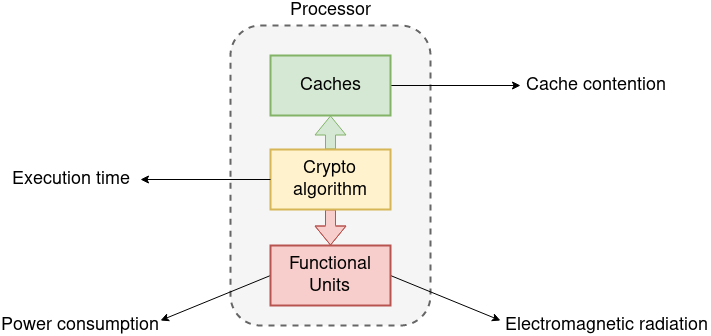
\includegraphics[width=0.7\textwidth]{side_channel.png}
    \caption[Data leakage sources]{A number of side channels which are capable of leaking data.}
    \label{fig:dls}
\end{figure}
\end{frame}

\subsection{Data dependent execution}
\begin{frame}[fragile]
\frametitle{Data dependent execution}

\begin{columns}[t]
    \column{0.49\textwidth}
        \textbf{Fast exponentiation algorithm used in RSA\footnote[frame]{\cite{cache_missing}}}
        \begin{lstlisting}[language={C}]
while(key > 0) {
    e = key % 2;

    Square();
    Reduce();
    if(e == 1) {
        Multiply();
        Reduce();
    }

    key >>= 1;
}
        \end{lstlisting}
    \column{0.49\textwidth}
        \textbf{S-box access used in AES\footnote[frame]{\cite{bern}}}
        \begin{lstlisting}[language={C}]
for(i=0; i<9; i++) {
    x = k;
    y = k ^ n;

    e = {S[x[1]]^1, S[x[2]],
         S[x[3]], S[x[0]]};
}
// Just for last round
y[0] = S[y[0]]^S[y[1]]^
       S[y[2]]^S[y[3]]^
        x[0];
        \end{lstlisting}
\end{columns}
\end{frame}

\subsection{Cache side channels}
\begin{frame}
\frametitle{Cache Side Channel}
\begin{enumerate}
    % \item Threads running in a single core use the same L1 caches. Processes on different cores of the same multi-core chip share L2 and L3 caches.
    \item Determine the cache-line accessed by victim using contention in shared cache.
    \item In set-associative cache design, that reveals a few bits of the address.
    \item For publicly available encryption libraries (OpenSSL), determine memory region of victim accesses.
    \item Using both these information, we can pinpoint exact address accessed by victim.
\end{enumerate}
\end{frame}

\begin{frame}
\frametitle{Prime+Probe}
\begin{figure}
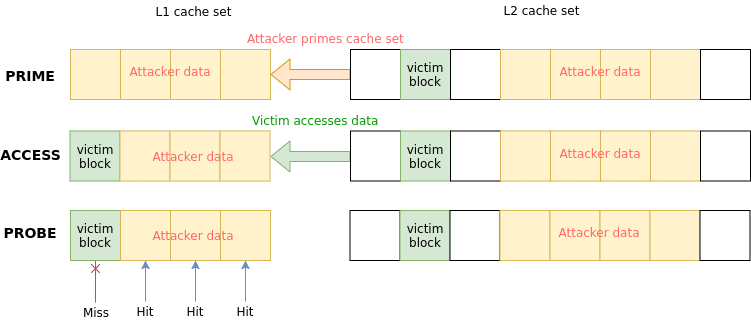
\includegraphics[width=0.9\textwidth]{prime_probe}
\caption{Working of Flush+Reload attack}
\end{figure}
\end{frame}

\begin{frame}
\frametitle{Flush+Reload}
\begin{figure}
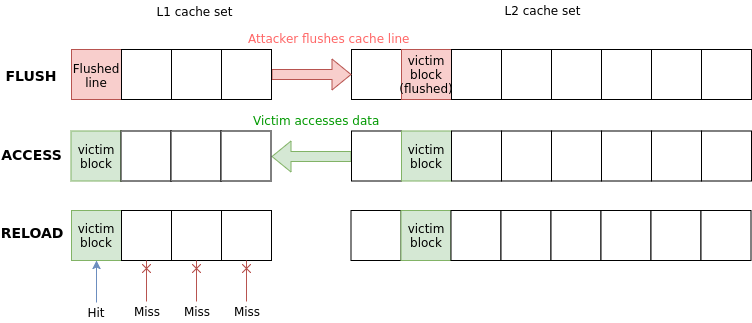
\includegraphics[width=0.9\textwidth]{flush_reload}
\caption{Working of Flush+Reload attack}
\end{figure}
\end{frame}

\begin{frame}
\frametitle{Flush+Reload on LLC}

\begin{columns}[c]
\column{0.6\textwidth}
\begin{figure}
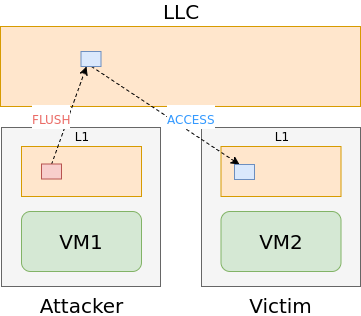
\includegraphics[width=\textwidth]{flush_reload_crossvm}
\caption{Cross-VM Flush+Reload Attack via LLC}
\end{figure}

\column{0.39\textwidth}
Virtual Machine environments are extensively used in cloud-computing
platforms to enable multiple different users share processors. VMs share a common host OS
which tries to optimise memory usage by performing page de-duplication. This allows VMs
    to share memory pages and hence enables hardware based side channels\footnote[frame]{\cite{cross_vm}}.
\end{columns}
\end{frame}

\subsection{Cache side channels on GPGPU}
\begin{frame}
\frametitle{Cache side channels on GPGPU}
Nvidia GPGPUs have recently started to support concurrent kernel execution at SM level, which allows multiple
programs to simultaneously use the GPGPU resource. In this shared context, one must
look at side channels which can be exploited.

\begin{figure}
    \centering
    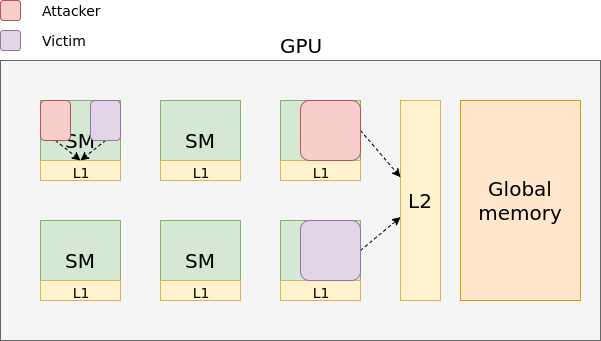
\includegraphics[width=0.8\textwidth]{gpgpu}
    \caption{Memory layout of GPGPUs}
\end{figure}
\end{frame}

\begin{frame}
\frametitle{GPGPU covert channel}
    Naghibijouybari et al in \footnote{\cite{naghi}} achieve communication speed of over 4Mbps
    using a combination of L1 cache contention and SFU contention as covert channels on multiple Nvidia
    GPGPU architectures. They have used the inherent parallelism in GPGPUs to multiply
    the speed of the created covert channels by opening parallel communication channels on
    each SM.
\begin{figure}
    \centering
    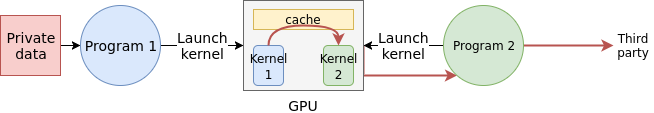
\includegraphics[width=0.95\textwidth]{covert_channel}
    \caption{Covert channel implementation on GPGPU}
\end{figure}
\end{frame}

\section{Reverse engineering implementation}
\begin{frame}[fragile]
\frametitle{Reverse engineer cache parameters}
    Knowing cache parameters is necessary for mounting any kind of side channel attacks on caches.
    This implementation of reverse engineering cache parameters is based on \footnote{\cite{wong}}. In that
    paper, Wong et al show how using a stride access pattern over an array to trigger a predictable number of cache-misses.

\begin{lstlisting}[caption={Generate array of given size with fixed stride pattern},language={C}]
size_t* array; // malloc beforehand
size_t t;

for (int i=0; i<array_size; i++) {
    t = i + STRIDE:
    if(t >= array_size) t %= STRIDE;
    array[i] = (size_t)array + sizeof(size_t)*t;
}
\end{lstlisting}

\end{frame}


\begin{frame}[fragile]
\frametitle{Reverse engineering cache parameters}
For measuring timing of the array access, \texttt{rdtsc} instruction is used to get a reading of the Time Step Counter before
and after accessing the array. The listing shows how to traverse the array
using the stride access data stored in it.
\begin{lstlisting}[caption={Timing measurement of stride access over the entire array},language={C}]
long start = __rdtsc();
size_t* next_ptr = &array[0];
for(int i=0; i<MAX_ITERS; i++) {
    next_ptr = *((size_t**)next_ptr);
}
long time = __rdtsc() - start;
\end{lstlisting}
\end{frame}

\begin{frame}
\frametitle{Result Plots}
Setup: GEM5 x86 atomic CPU. L1 data cache 1KB, 2-way, 64B line size.
\begin{figure}
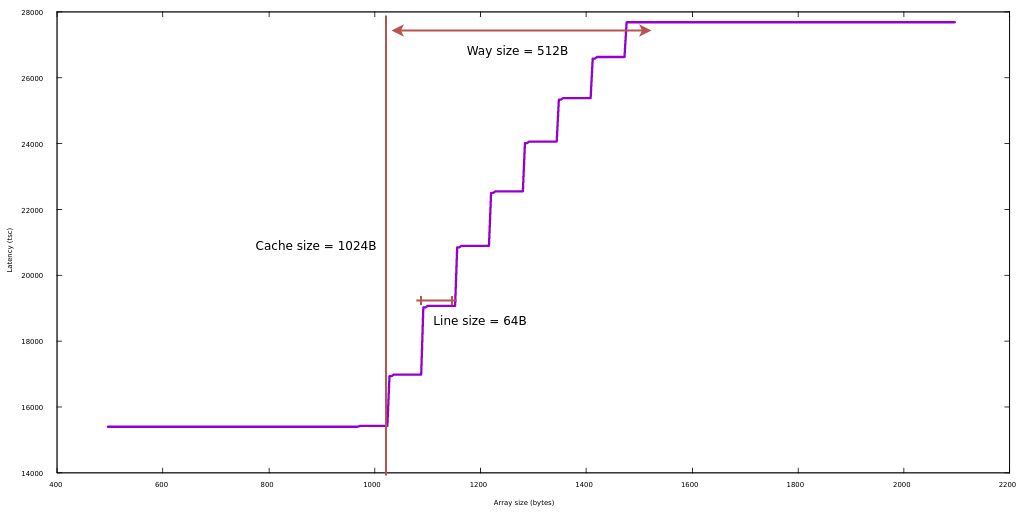
\includegraphics[width=0.9\textwidth]{reverse_eng_1kb}
\caption{Latency vs Array Size plot}
\end{figure}
\end{frame}

\begin{frame}
\frametitle{Result Plots}
Setup: GEM5 x86 atomic CPU. L1 data cache 16KB, 4-way, 64B line size.
\begin{figure}
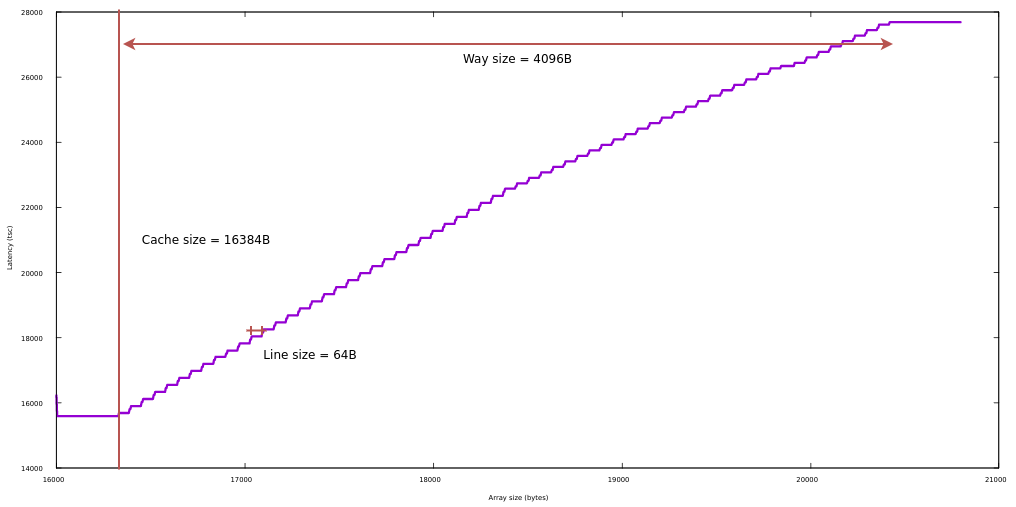
\includegraphics[width=0.9\textwidth]{reverse_eng_16kb}
\caption{Latency vs Array Size plot}
\end{figure}
\end{frame}

\begin{frame}
\frametitle{Result Plots}
Setup: Intel Skylake x86\_64 i5-6500. L1 data cache 32KB, 8-way, 64B line size.
\begin{figure}
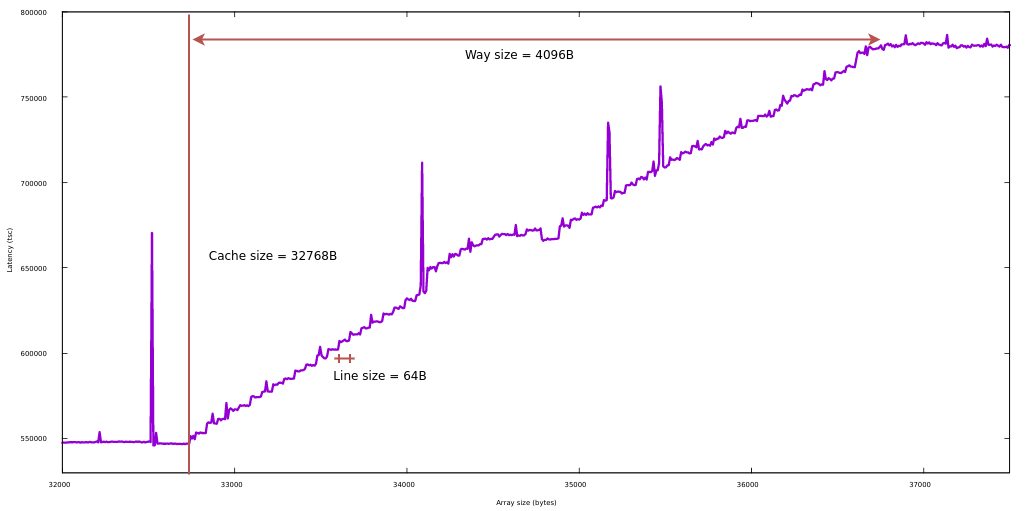
\includegraphics[width=0.9\textwidth]{reverse_eng_32kb}
\caption{Latency vs Array Size plot}
\end{figure}
\end{frame}

\section{Mitigations against Cache side channel}

\begin{frame}
\frametitle{Mitigations against cache side channel}
\begin{itemize}
    \item Change the implementation of each encryption algorithm to avoid leaks.
    \item Only possible for known attacks and unavoidable for any software to not leave fingerprint in shared resources.
    \item Change hardware design of caches so that one process doesn’t affect other processes via its cache accesses in a predictable way.
    \item Intentionally pollute cache to add noise in side channel measurements.
\end{itemize}
\end{frame}

\subsection{Partition-locked cache}

\begin{frame}
\frametitle{Partition-Locked cache}
Naive cache partitioning would equally split cache for all threads.
    Such a partitioned cache will let only one process access a single partition at a time \footnote{\cite{part_cache}}.
    Wang et al have proposed a dynamically partitioned cache in \footnote{\cite{wang}}.
\begin{figure}[h]
\centering
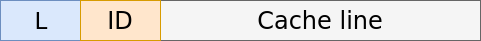
\includegraphics[width=\textwidth]{pl-cache}
\caption{Partition-Locked cache - single cache line}
\end{figure}
PLCache requires addition of special locked-load/store instructions to the ISA.
This also means OS has to look over
which process gets to use them as a fairness measure.
\end{frame}

\subsection{Random-permutation cache}

\begin{frame}
\frametitle{Random-Permutation Cache}
Random-permutation cache is another cache design proposed by Wang et al. They
have added a redirection step in the address decoder of caches which uses a random permutation table.
\begin{figure}[h]
\centering
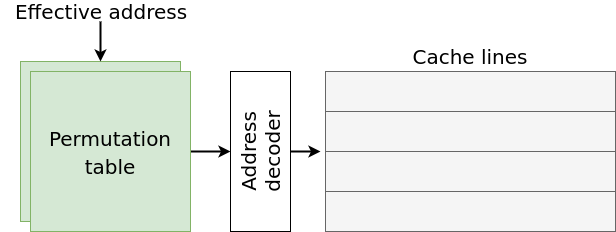
\includegraphics[width=0.7\textwidth]{rp-cache}
\caption{Random-permutation cache}
\end{figure}
RPcache is able to mark data using "Lock" bits by copying page protection bit.
Drawback of RPCache is the added step in address decoding.
1 or 2 cycle latency increase will drastically change performance of L1.
\end{frame}

\subsection{Disruptive prefetching}
\begin{frame}
\frametitle{Disruptive Pre-fetching}
\begin{itemize}
    \item Fuchs et al in \footnote{\cite{disruptive_prefetch}} introduce additional steps to the pre-fetchers to increase the randomness
in the loaded memory address.
\item Randomise the pattern sequence and stride value to intentionally pollute the cache with unnecessary data.
\item Slightly degrades the performance of non-malicious programs, but terribly disrupt side channel.
\item Prime+Probe attack will not know whether the victim or the pre-fetcher evicted its block.
\item Flush+Reload would get false cache hits which were not caused by the victim.
\end{itemize}
\end{frame}

\subsection{Context Sensitive Decoding}
\begin{frame}
\frametitle{Context Sensitive Decoding}
A lot of modern processors use decoders to convert from ISA to an internal instruction
    representation. Taram et al explore in \footnote{\cite{csd}} if a custom decoder can insert decoy
instructions to improve security.
\begin{figure}
\centering
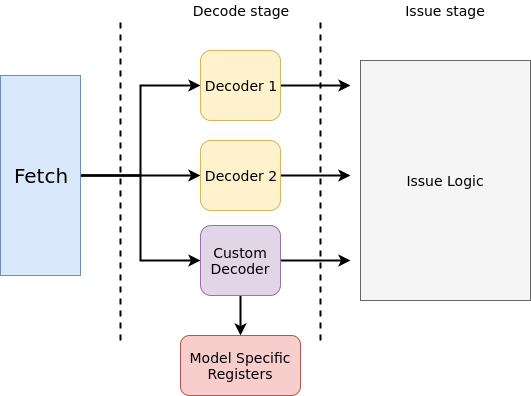
\includegraphics[width=0.4\textwidth]{csd}
\caption{Custom decoder for Context Sensitive Decoding}
\end{figure}
Decoy instructions pollute the cache by running decoy loads and
disrupt attackers attempting side channel attacks on the cache.
\end{frame}

\section{ROB based Side Channel}
\begin{frame}
\frametitle{Hypothetical ROB based Side Channel}
\begin{itemize}
    \item Reorder buffer is used by Out-of-Order cores for in-order retirement.
    \item In SMT cores, fairness policy ensures that roughly equal instructions are retired for all threads to maintain equal IPC.
    \item Simple implementation is to share retire pipeline width equally among threads.
    \item But when one thread is stalled, other thread will use full pipeline width to retire.
    \item IPC of other threads will see a slight increase.
    \item Data-dependent branch misses and cache misses can be infered from IPC information.
\end{itemize}
\end{frame}

\begin{frame}
\frametitle{Hypothetical ROB based Side Channel}
\begin{figure}
\centering
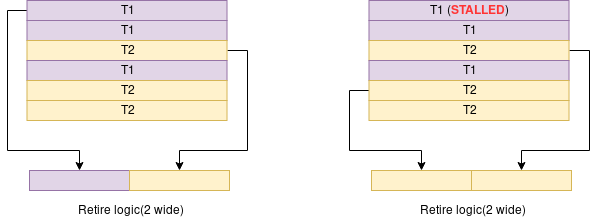
\includegraphics[width=0.8\textwidth]{rob_side_channel}
\caption{Reorder buffer for SMT. When T1 is stalled T2 retires twice as many instructions.}
\end{figure}
\end{frame}

\section{Conclusion}
\begin{frame}
    \frametitle{Conclusion and future work}
\begin{itemize}
\item Modern hardware features have introduced leakages in the processor which is a security concern.
\item GPGPUs are being targeted as a new domain of security leaks.
\item Hardware design needs to take into account these kind of security leaks.
\item Explore other shared resources apart from caches as potential leakage sources.
\end{itemize}
\end{frame}

\begin{frame}
\Huge{\centerline{The End}}
\end{frame}

\begin{frame}[allowframebreaks]
    \frametitle<presentation>{For Further Reading}

    \begin{thebibliography}{10}
        \bibitem[D. Page, Theoretical Use of Cache Memory as a Cryptanalytic Side-Channel]{cache_side_channel}
Theoretical Use of Cache Memory as a Cryptanalytic Side-Channel
, D. Page, Department of Computer Science, University of Bristol

        \bibitem[C. Percival, Cache missing for fun and profit]{cache_missing}
            Cache Missing for Fun and Profit, Colin Percival

        \bibitem[D. J. Bernstien, Cache-timing attacks on AES]{bern}
            Cache-timing attacks on AES, D.J. Bernstien

        \bibitem[Chenglu Jin, Side Channel Attacks]{side_channel_intro}
Side Channel Attacks, Chenglu Jin, Department of Electrical \& Computer Engineering, University of Connecticut

        \bibitem[Wait a minute! A fast, Cross-VM attack on AES - RAID'14]{cross_vm}
Gorka Irazoqui, Mehmet Sinan Inci, Thomas Eisenbarth, Berk Sunar, Wait a minute! A fast, Cross-VM attack on AES

\bibitem[D. Page - Partitioned Cache Architecture as a Side-Channel Defence Mechanism]{part_cache}
D. Page, {\it Partitioned Cache Architecture as a Side-Channel Defence Mechanism}

        \bibitem[New Cache Designs for Thwarting Software Cache-based Side Channel Attacks - ISCA'07]{wang}
Z. Wang and R. B. Lee, New Cache Designs for Thwarting Software Cache-based Side Channel Attacks, ISCA'07

        \bibitem[A novel cache architecture with enhanced performance and security - MICRO'08]{newcache}
Z. Wang and R. B. Lee. A novel cache architecture with enhanced performance and security. In Proceedings of the 41st Annual Inter­national Symposium on Microarchitecture, MICRO 2008

        \bibitem[Disruptive prefetching: impact on side-channel attacks and cache designs - SYSTOR'15]{disruptive_prefetch}
Adi Fuchs and Ruby B. Lee. 2015. Disruptive prefetching: impact on side-channel attacks and cache designs. In Proceedings of the 8th ACM International Systems and Storage Conference (SYSTOR '15)

        \bibitem[Constructing and characterizing covert channels on GPGPUs - MICRO-50]{naghi}
            Hoda Naghibijouybari, Khaled N. Khasawneh, and Nael Abu-Ghazaleh. Constructing and characterizing covert channels on GPGPUs - MICRO'50

        \bibitem[Demystifying GPU microarchitecture through microbenchmark - ISPASS]{wong}
            Henry Wong, M. M. Papadopoulou, Maryam Sadooghi-Alvandi, and Andreas Moshovos. 2010. Demystifying GPU microarchitecture through microbenchmark - ISPASS'10

        \bibitem[Mobilizing the Micro-Ops: Exploiting Context Sensitive Decoding for Security and Energy Efficiency - ISCA'18]{csd}
        Mohammadkazem Taram, Ashish Venkat, Dean Tullsen, Mobilizing the Micro-Ops: Exploiting Context Sensitive Decoding for Security and Energy Efficiency - ISCA'18
    \end{thebibliography}
\end{frame}

%----------------------------------------------------------------------------------------

\end{document}
